\section{Описание подхода}

TalkNet разбивает генерацию мэл-спектрограммы из текста на два отдельных модуля. Первый модуль, предсказатель длительности, выравнивает входные графемы по времени относительно звуковой дорожки (или мэл-спектрограммы, что то же самое так так длина мэл-спектрограммы линейно зависит от длины аудио). Второй модуль, генератор мэл-спектрограмм, производит генерацию из выровненных по времени входных символов (Рисунок~\ref{fig:arch}). Мы используем конволюционные модели прямого вывода (feed-forward) для обоих модулей, поэтому как обучение, так и вывод не являются авторегрессионными. Это позволяет гораздо быстрее обучаться и делать вывод по сравнению с авторегрессионными моделями. Для обучения предсказателя длительности графем мы извлекли истинностые длительности из выхода CTC предварительно обученной модели разпознавания речи (Automatic-Speech-Recognition, ASR).

\subsection{Извлечение истинных длительностей графем}

Центральная идея TalkNet заключается в использовании модели ASR на основе Connectionist Temporal Classification (CTC) функции ошибки для извлечения выравниваний графем. CTC присваивает вероятность каждому из символов алфавита и использует вспомогательный пустой символ $\sim$. Первым шагом мы схлопываем соседние повторяюшиеся символы в выводе, подсчитывая таким образом длительность каждого символа. Пустой символ выступает как промежуточное состояние между двумя соседними графемами, и его длительность соответствует длительности перехода от одного символа к другому. Для каждого временного шага мы выбираем наиболее вероятный символ из выходных данных CTC (Рисунок~\ref{fig:ctc}).

\begin{figure}[!ht]
\centering
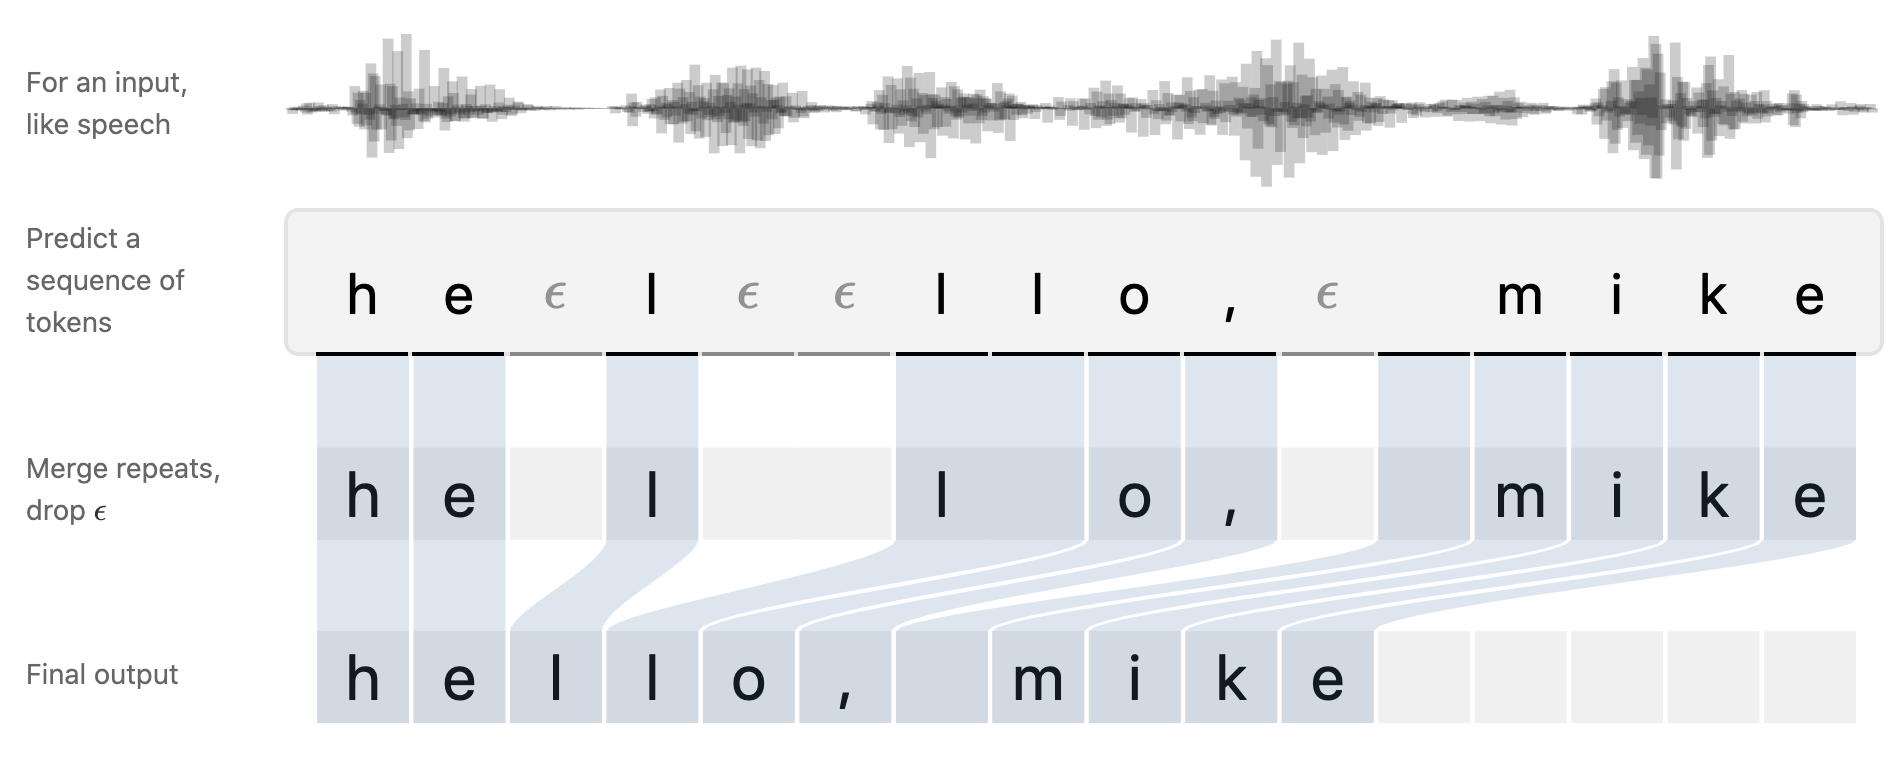
\includegraphics[width=1.0\textwidth]{images/snippets/ctc.png}
\caption{Пример работы CTC алгоритма~\cite{hannun2017sequence}. Соседние буквы схлопываются, а $\epsilon$ ($\sim$ в нашей нотации) служит разделительным вспомогательным символом.}
\label{fig:ctc}
\end{figure}

CTC -- это функция ошибки, используемая для этапа обучения. Поэтому, выход CTC часто бывает неточен. Однако, задача ASR решена намного лучше TTS, поэтому ошибка все еще меньше. Мы выравниваем выход CTC с истинным отрывком текста для того чтобы максимально устранить влияние ошибки. Мы используем функцию \textit{pairwise2} из пакета Biopython~\cite{biopython}, которая выравниваем два строковых представления побуквенно, используя наименьшее количество операции добавления и удаления символов. Затем мы удаляем все неправильные символы в выводе CTC, добавля их длительность к ближайшему пустому, а также добавляем недостающие символы и устанавливаем их длительность в $0$. Затем для всех символов с предсказанной длительностью 0 мы устанавливаем длительность в 1, вычитая 1 из почти самого большого соседнего $\sim$, чтобы сумма всех длительностей графемы была равна длине мэл-спектрограммы (Рисунок~\ref{fig:alignment}).

\begin{figure}[!ht]
\centering
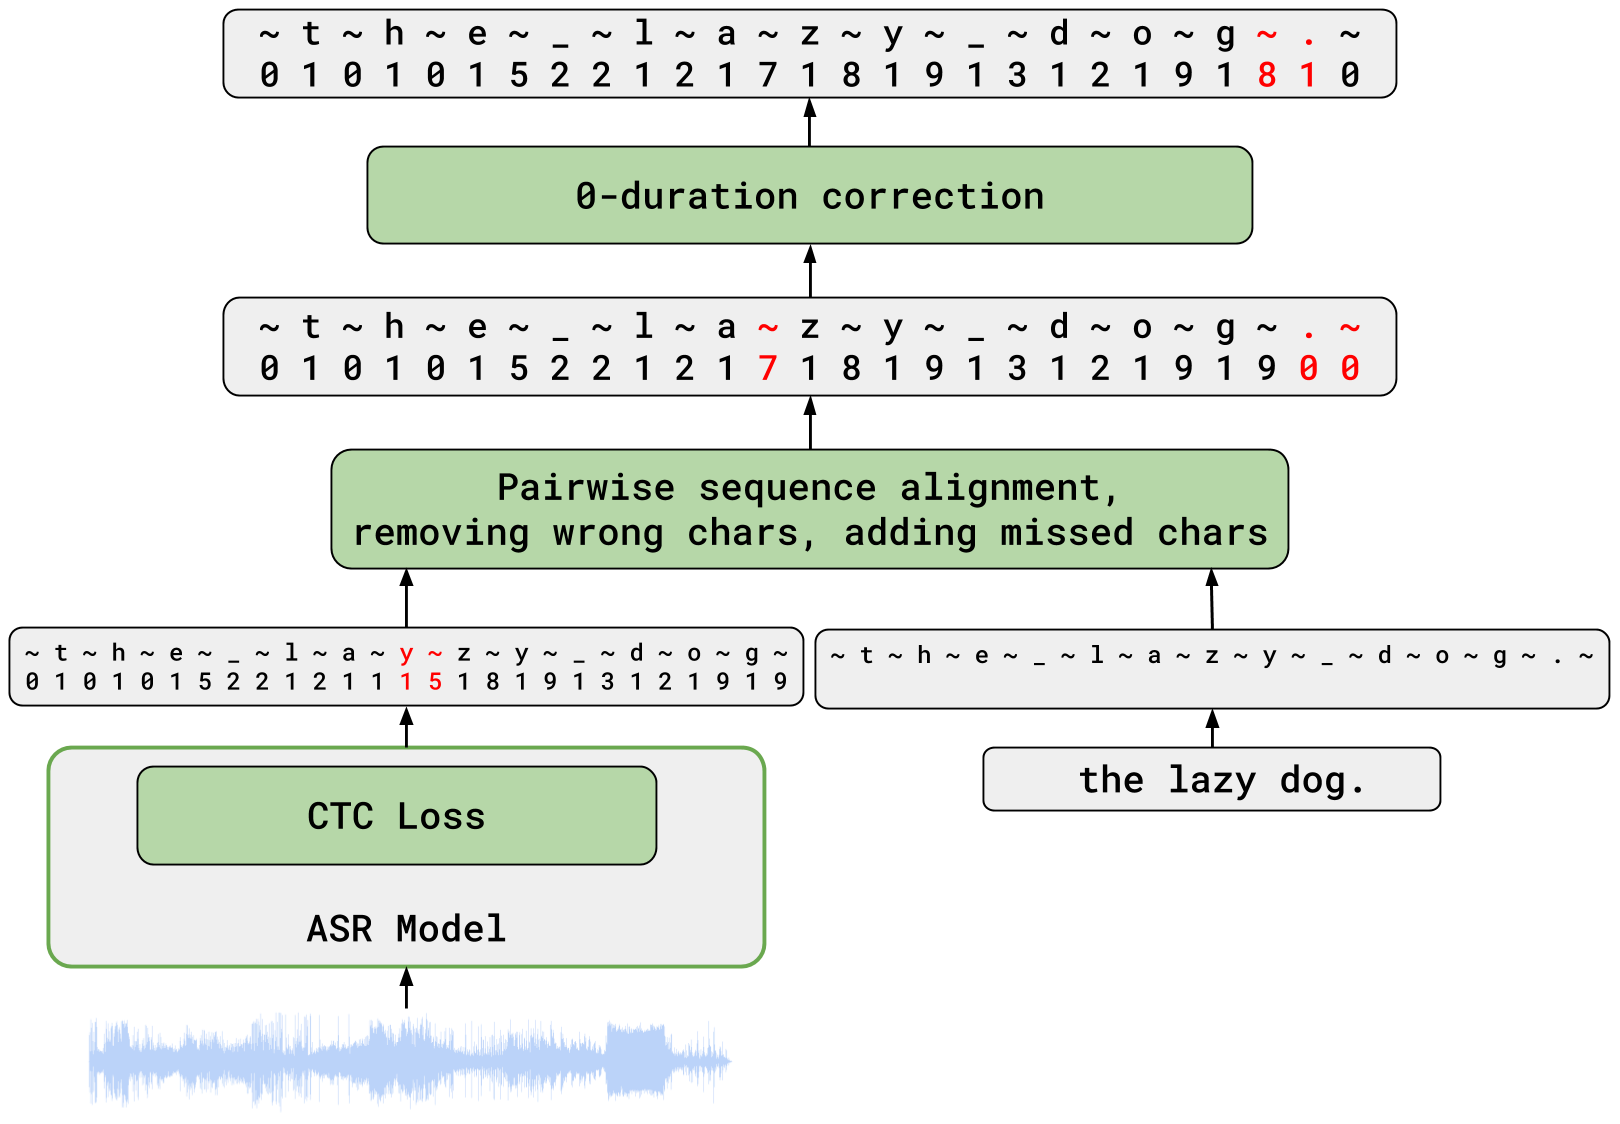
\includegraphics[width=1.0\textwidth]{images/alignment.png}
\caption{Извлечение длительности графемы из вывода CTC. Мы используем $\sim$ для обозначения пустого символа.}
\label{fig:alignment}
\end{figure}

В качестве модели с CTC выводом для задачи разпознования текста (ASR) мы используем QuartzNet~\cite{quartznet}. QuartzNet (Рисунок~\ref{fig:qn}) -- это полностью-коволюционная нейронная архитектура, основными достоинствами которой являются:
\begin{itemize}
    \item Низкое количество параметров (около 18 миллионов), которое было достигнуто за счет использования depthwise separable~\cite{kaiser2017depthwise} конволюций, являющихся математическим приближение обычных конволюций.
    \item Простая неавторегрессионная архитектура с базовыми операциями из глубокого обучения (конволюции, нелинейности, батч-нормализация и дропаут), позволяющяя ускорить процесс обучения и вывода (inference).
    \item CTC функция в качестве функции ошибки в декодере, которая не содержит допольнительных параметров и обеспечивает быстрый вывод.
\end{itemize}

\begin{figure}[!ht]
\centering
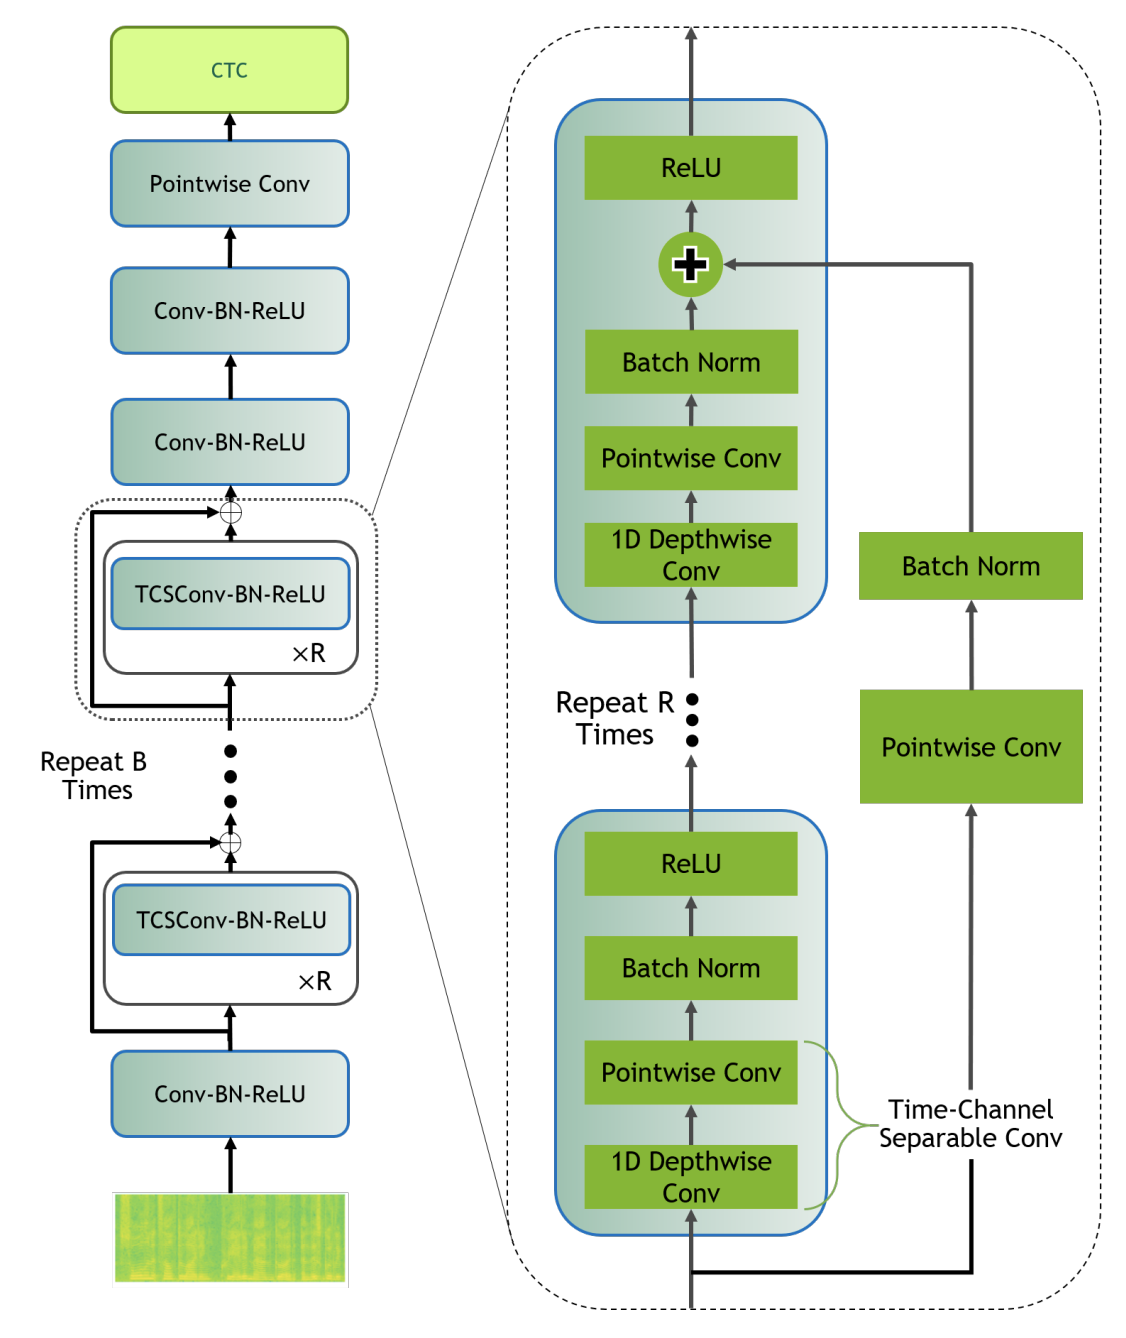
\includegraphics[width=1.0\textwidth]{images/qn.png}
\caption{Архитектура QuartzNet 15x5}
\label{fig:qn}
\end{figure}

Для получения истинных длительностей графем мы используем QuartzNet 15x5 (15 блоков по 5 повторений). Выход такой модели по длине в 2 раза меньше входной мэл-спектрограммы. Причина -- в самой первой конволюции выставлен параметр $\texttt{stride}=2$ (Рисунок~\ref{fig:stride-2}). QuartzNet использует удвоение шага в самом начале, так как для любого примера длина выходного текста как минимум в два раза меньше длины мэл-спектрограммы, поэтому такой трюк позволяет сократить количество вычислений вдвое. Однако, это так же уменьшает длительность каждого символа в выходе CTC. Чтобы сравнять сумму длительностей с длиной мэла, мы модифицируем QuartzNet, устанавливая $\texttt{stride}=1$ для первого слоя. Заметим так же что это не убирает возможность воспользоваться предобученной моделью, загрузив веса перед обучением для дообучения (fine-tuning) -- размеры, форма и количество ядер (kernels) конволюций остается неизменным. Соотвестсвенно, не изменяются и размеры матриц и векторов с весами.

\begin{figure}[!ht]
\centering
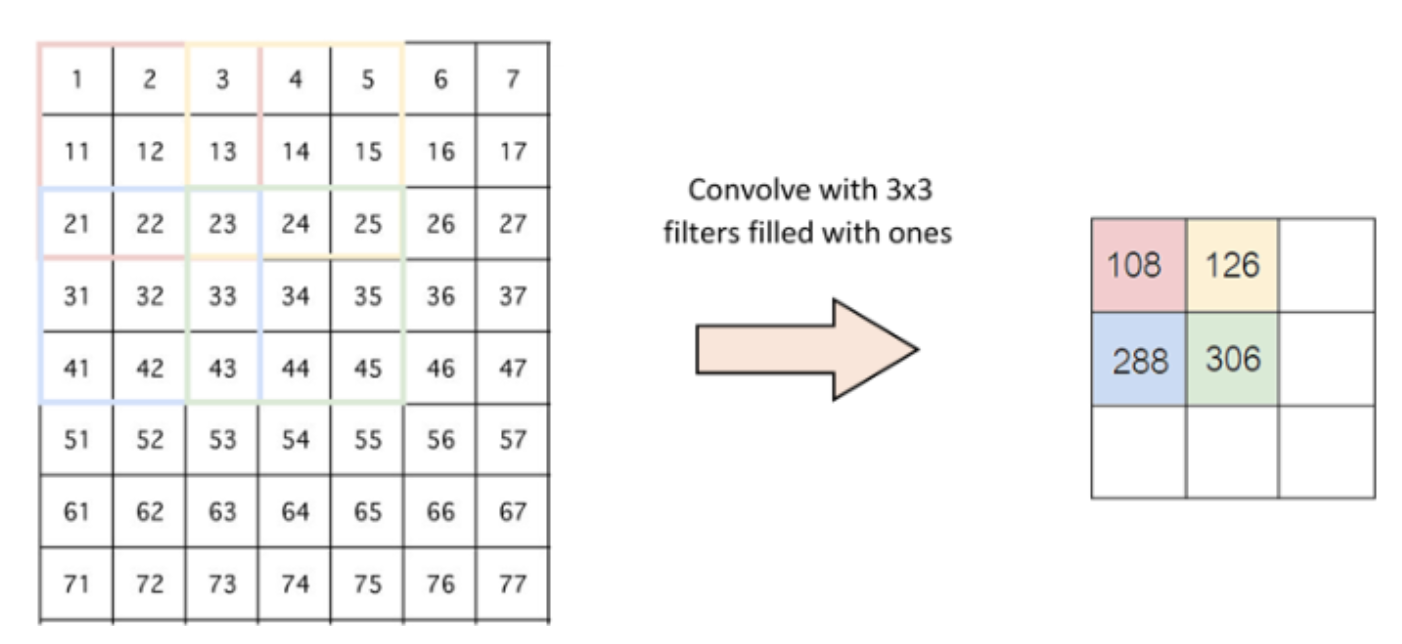
\includegraphics[width=1.0\textwidth]{images/snippets/stride-2.png}
\caption{Пример работы конволюций с удвоенным шагом}
\label{fig:stride-2}
\end{figure}

Мы дообучаем QuartzNet 15x5 на данных из датасета LibriTTS~\cite{libritts}. LibriTTS это набор данных из того же источника, что и LibriSpeech, на котором успешно обучался оригинальный QuartzNet. Однако, LibriTTS использует другую обработка данных, которая более подходит для задач генерации речи, нежели разпознования речи. В частности, LibriTTS обрезает отрывки аудио по большим паузам, оставляет всю пунктуацию нетронутой (для экспрессивности речи), а также разворачиваем некоторые числа и буквенные сокращения. Для токенизации входного текста (разбиения на символы) мы также оставляем всю пунктуацию, давая возможность CTC самому назначит длительность каждому сивмолу. При дообучении QuartzNet на LibriTTS мы достигаем побуквенной ошибки (Char-Error-Rate, CER) порядка $4.51\%$ на части dev-clean и порядка $3.54\%$ на тестовой части LJSpeech~\cite{ljspeech}. Выравнивание, полученное из CTC, используется для обучения предиктора длительности графемы.

Таким образом, вместо того чтобы использовать другую преодобученную TTS модель в качестве учителя для получения длительностей графем, как это делалось в модели FastSpeech~\cite{fastspeech}, мы представляем метод в котором используется ASR модель. Ошибка, получаемая в CTC гораздно меньше ошибки при генерации речи, поэтому такой способ позволяет снять жесткое ограничение на качество, задаваемой моделью учителя.

\subsection{Grapheme duration predictor}

This model predicts the length of the mel-spectrogram part corresponding to each gra\-pheme in the input including punctuation. First, the grapheme duration predictor inserts a blank symbol $\sim$ between every two input characters. Next, it predicts the duration for each input character. We expand the sequence of input characters by repeating each character according to the predicted duration  (Figure~\ref{fig:durs}).

\begin{figure}[!ht]
\centering
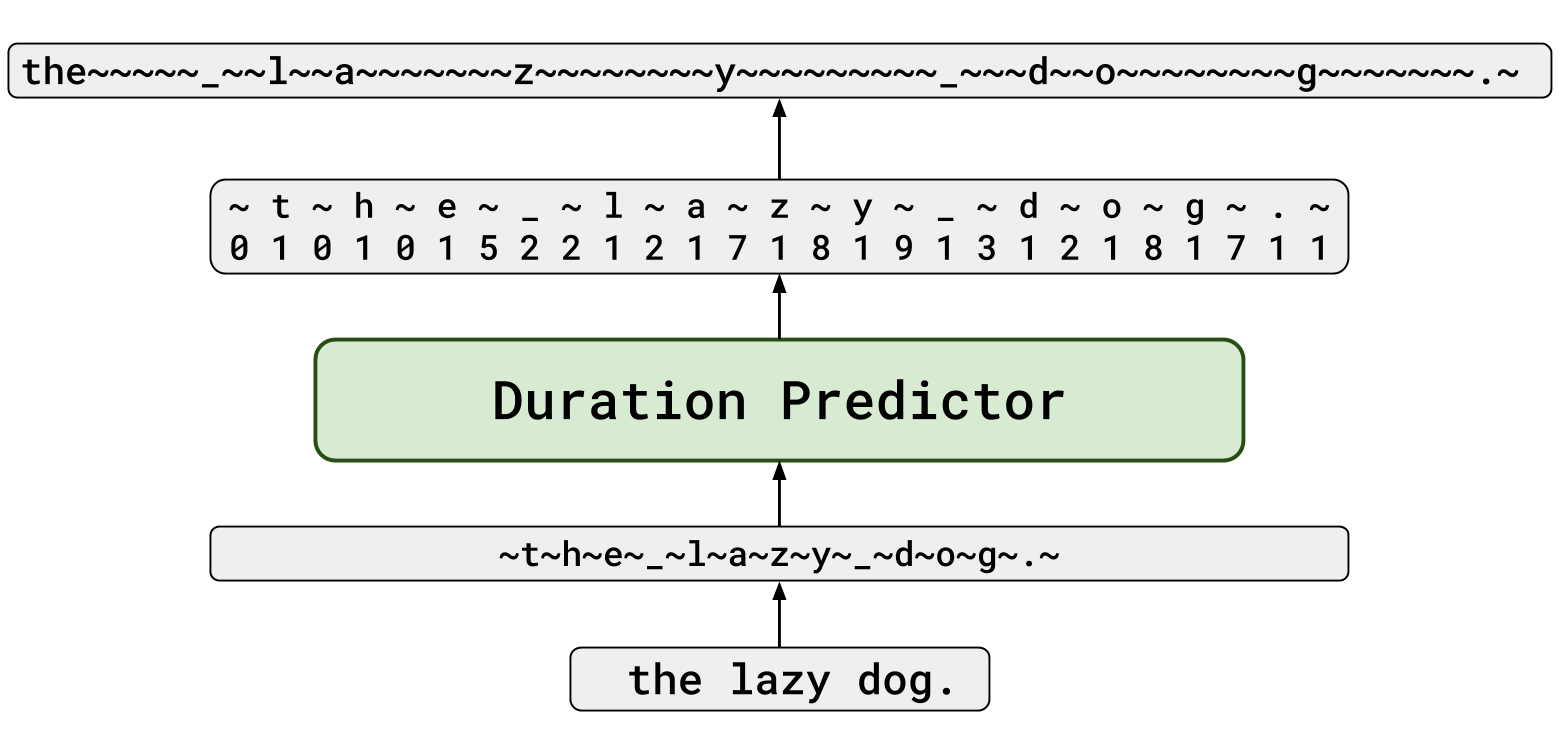
\includegraphics[width=1.0\linewidth]{images/durs.png}
\caption{Grapheme duration prediction.}
\label{fig:durs}
\end{figure}

The grapheme duration predictor model is a 1D time channel separable convolutional NN based on QuartzNet architecture~\cite{quartznet}. The model has $5$ residual blocks with 5 sub-blocks per block. A sub-block consists of a 1D time-channel separable convolution, a 1x1 pointwise convolutions, batch norm, ReLU, and dropout (see Figure~\ref{fig:qn-block}). There are two additional layers: the grapheme embedding layer, and a $1x1$ convolutional layer before loss function (see Table~\ref{tab:durs-model}).

\begin{figure}[!ht]
\centering
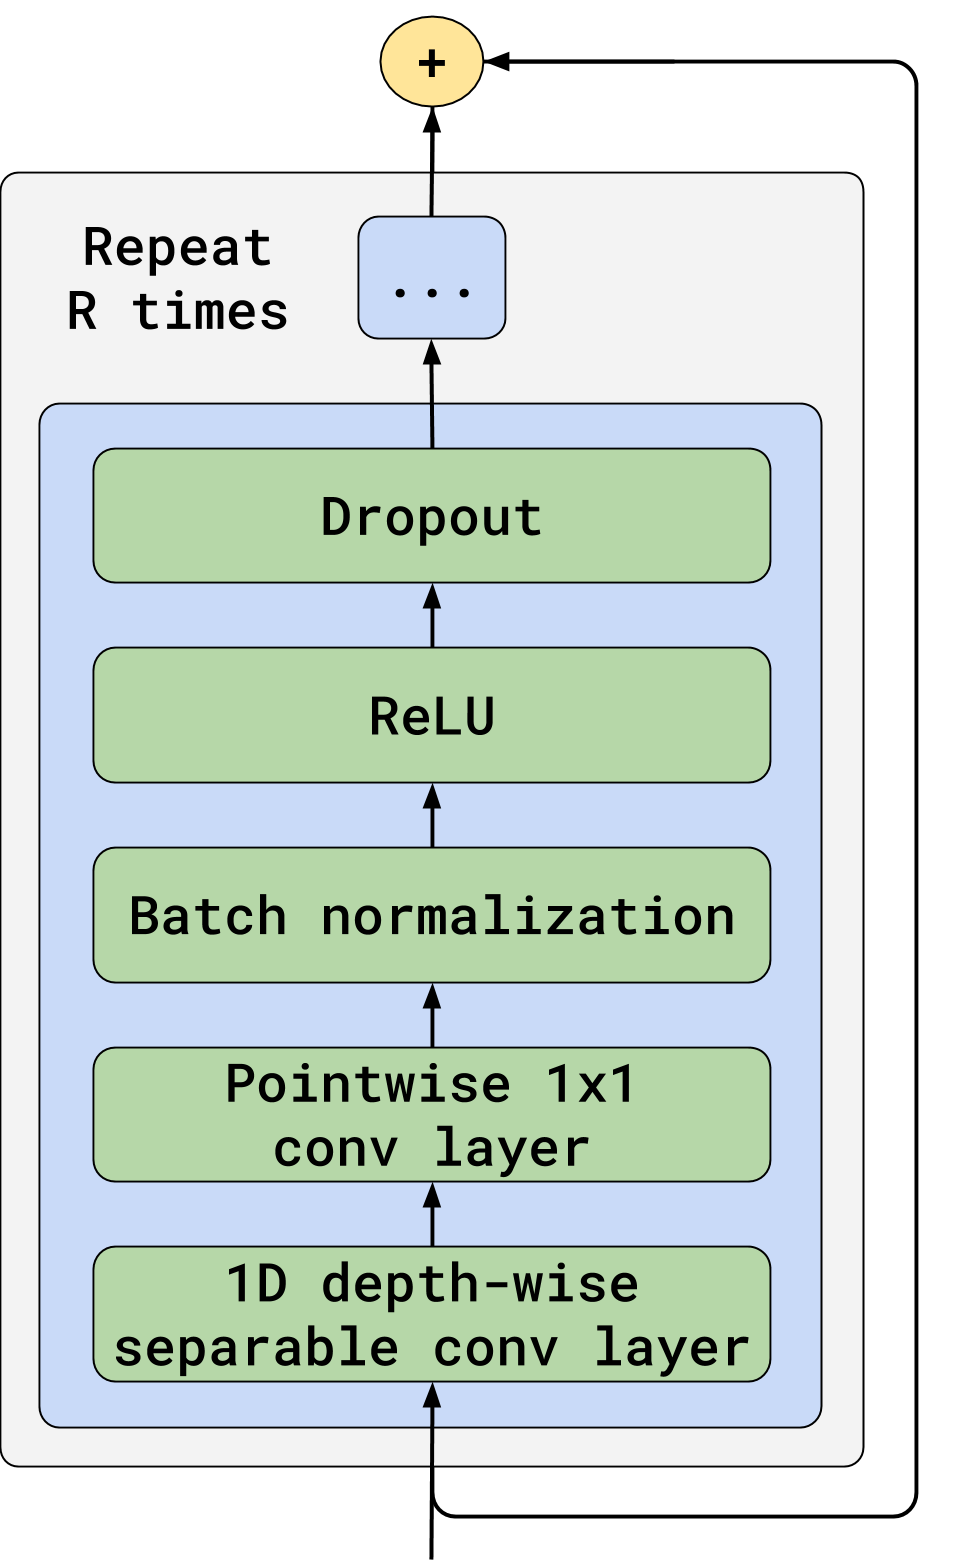
\includegraphics[width=0.8\linewidth]{images/qn-block.png}
\caption{Basic QuartzNet block. Both grapheme duration predictor and mel-spectrogram generator are 1D time-channel convolutional networks based on QuartzNet~\cite{quartznet}.}
\label{fig:qn-block}
\end{figure}

We train a duration predictor using $L_2$ loss with logarithmic targets, similar to~\cite{fastspeech}. We also tried cross-entropy (XE) loss with each class corresponding to the character duration. We used a log scale for large durations since grapheme duration distribution has a long tail (Figure~\ref{fig:durs-dist}). Cross entropy has slightly higher accuracy (see Table~\ref{tab:durs-results}). We choose $L2$ since a speech generated with L2 loss got slightly higher mean-opinion-score (MOS) in our evaluation studies.

\begin{figure}[!ht]
\centering
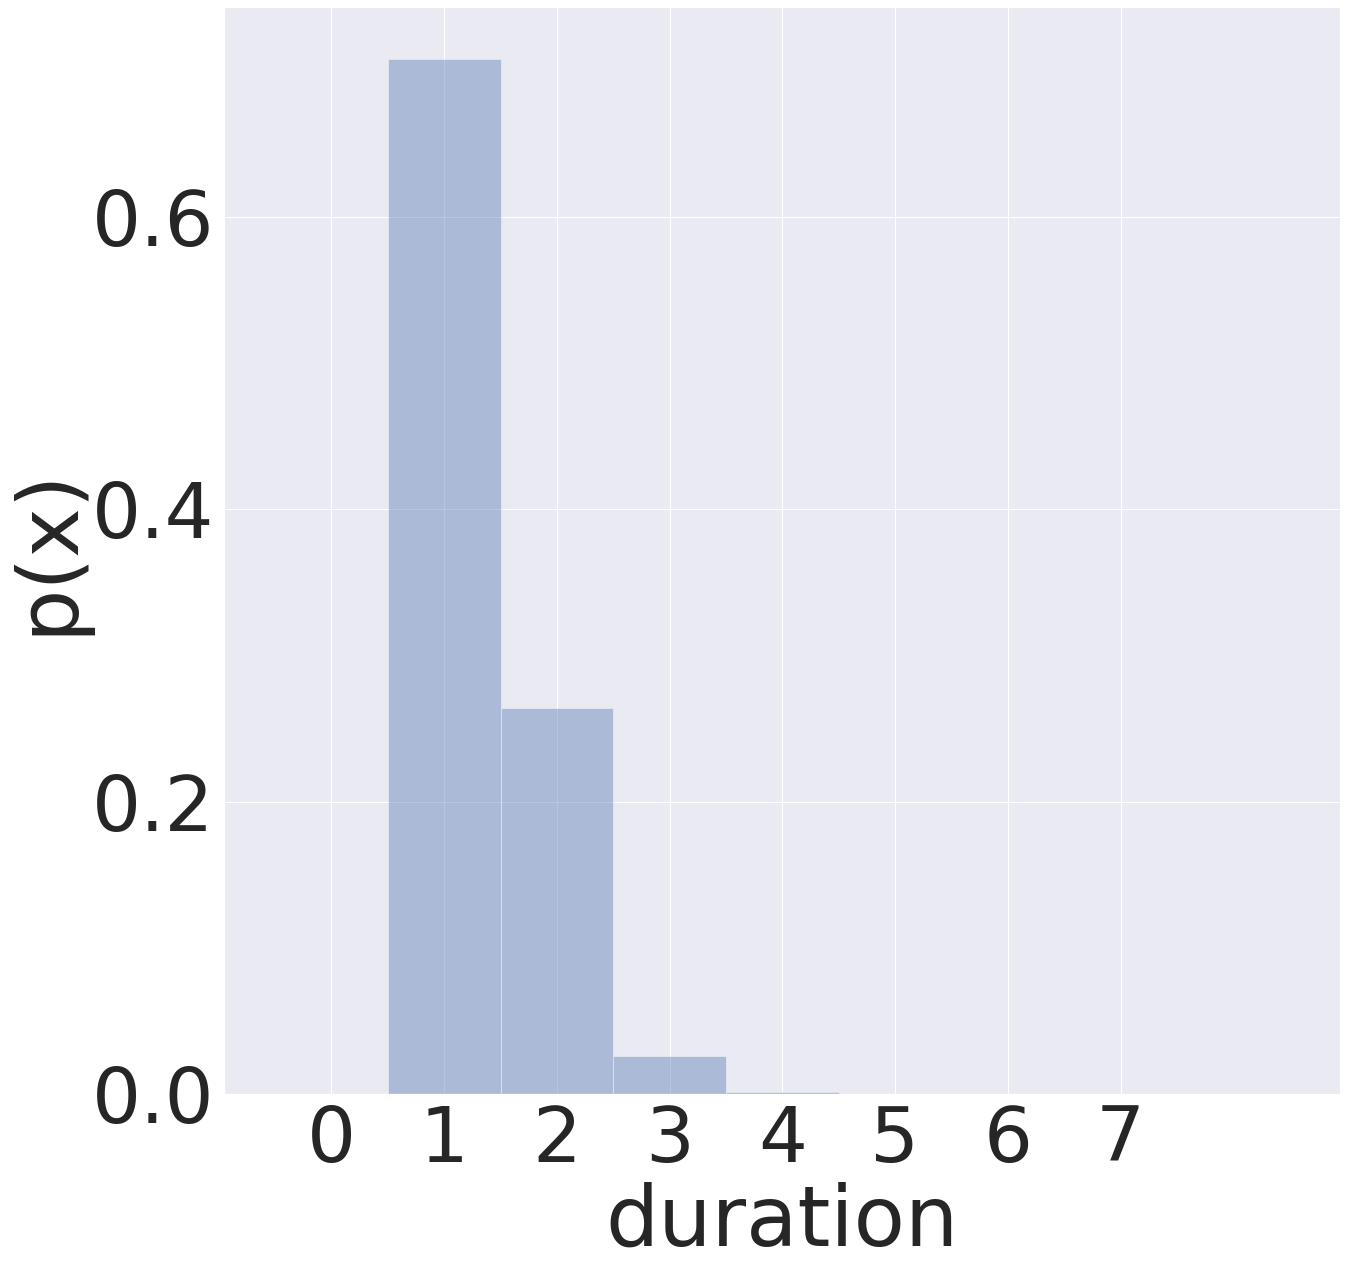
\includegraphics[width=.48\linewidth]{images/durs-dist.png}
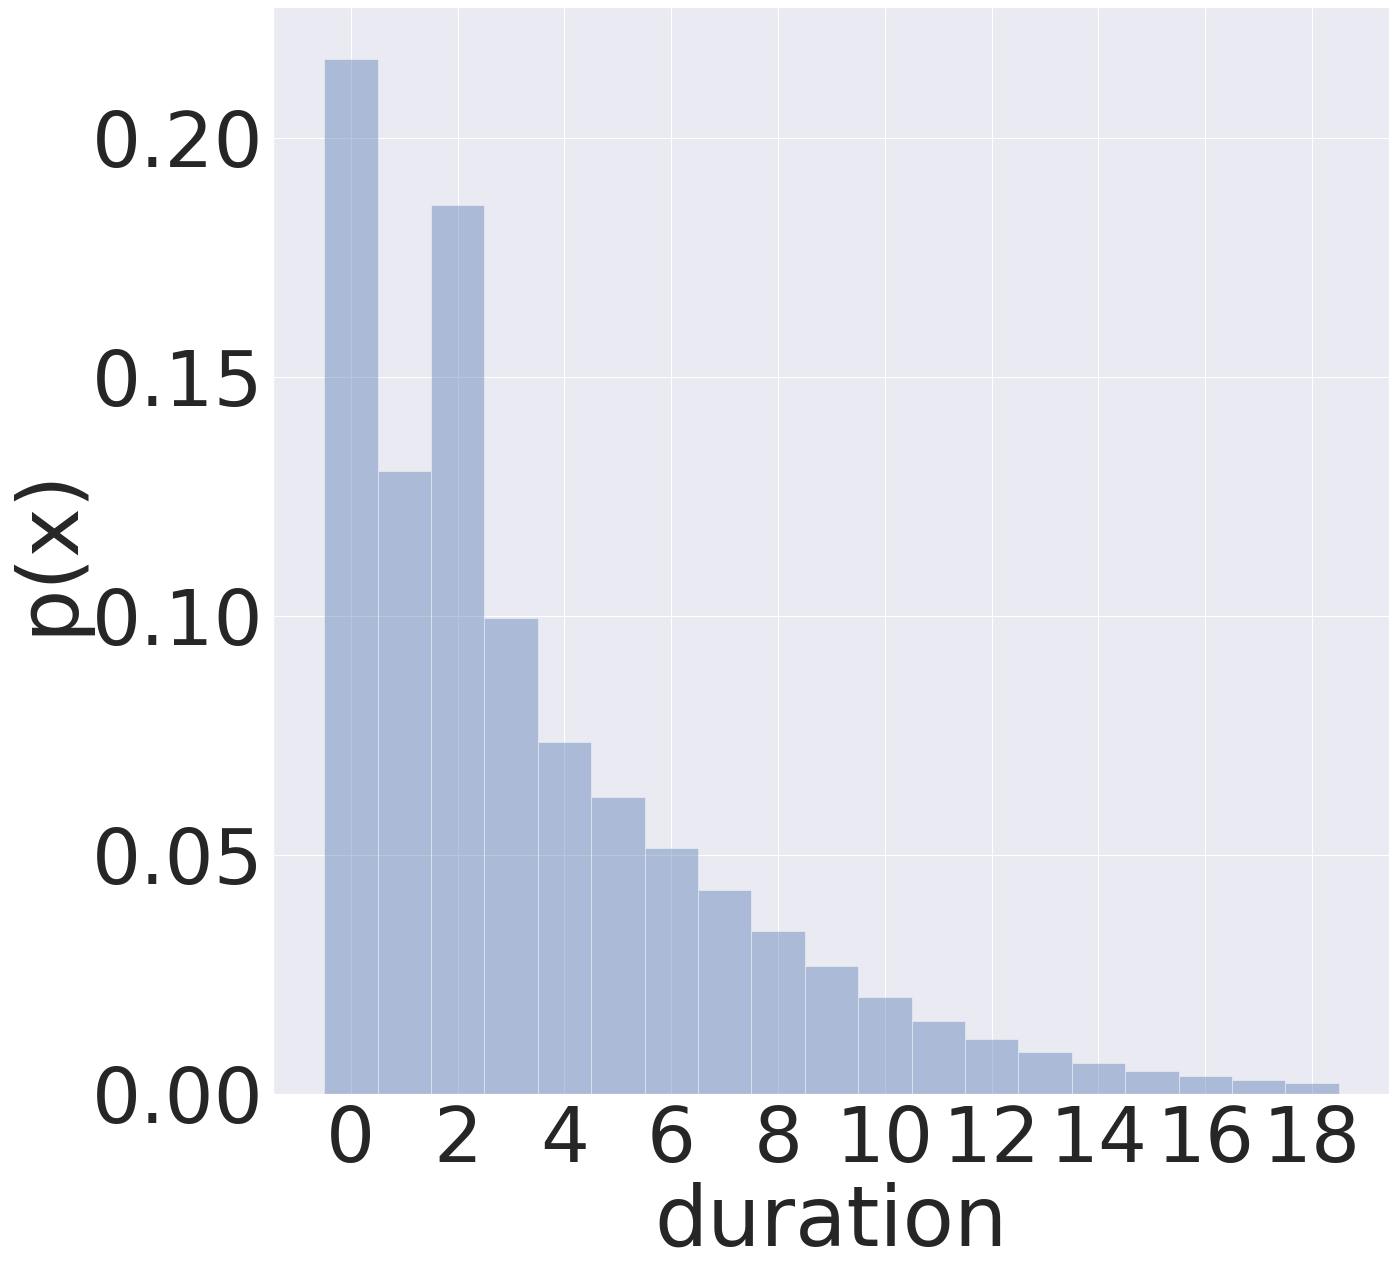
\includegraphics[width=.48\linewidth]{images/blanks-dist.png}
\caption{The duration's distribution for characters (left) and for blanks (right) based on CTC output for LJSpeech dataset. The maximum duration for characters is $7$, and for blanks -- $493$.}
\label{fig:durs-dist}
\end{figure}

\begin{table}[!ht]
\centering
\scalebox{1.0}{
\begin{tabular}{c c c c c} 
\toprule
\textbf{Block} &
\textbf{\thead{\# Sub\\Blocks}} &
\textbf{\thead{\# Output\\Channels}} &
\textbf{Kernel Size} &
\textbf{Dropout} \\
\midrule
Embed & 1 & 64  & 1 & 0.0  \\
Conv1 & 3 & 256 & 3 & 0.1  \\
$B_1$ & 5 & 256 & 5 & 0.1  \\
$B_2$ & 5 & 256 & 7 & 0.1  \\
$B_3$ & 5 & 256 & 9 & 0.1  \\
$B_4$ & 5 & 256 & 11 & 0.1 \\
$B_5$ & 5 & 256 & 13 & 0.1 \\
Conv2 & 1 & 512 & 1 & 0.1  \\
Conv3 & 1 & $32$ & 1 & 0.0 \\
\midrule
\textbf{Params, M} & & & & \textbf{2.3} \\
\bottomrule
\end{tabular}
}
\caption{Grapheme duration predictor is based on QuartzNet 5x5.}
\label{tab:durs-model}
\end{table}

\begin{table}[!ht]
\centering
\scalebox{1.0}{
\begin{tabular}{c c c c c c c} 
\toprule
\textbf{Method} &
\textbf{MSE} &
\textbf{Accuracy, $\%$} &
$\mathbf{|P - T| \leq 1}$ &
$\mathbf{|P - T| \leq 3}$\\
\midrule
$L_2$ & 7.81 & 67.69 & 91.90 & 97.17 \\
XE & 10.46 & 69.42 & 92.90 & 97.40 \\
\bottomrule
\end{tabular}
}
\caption{Duration's predictor results, LJSpeech test set. $P$ -- predicted, $T$ -- target.}
\label{tab:durs-results}
\end{table}

\subsection{Mel-spectrogram generator}

The second module generates mel-spectrogram from the expanded text. The mel-spectro\-gram generator is a 1D convolutional network based on the same QuartzNet architecture. It has $9$ blocks with 5 sub-blocks (see Table~\ref{tab:mels-model}). The mel-spectrogram generator was trained with a mean square error (MSE) loss.

Instead of allocating a separate embedding for blank symbol, we use a linear combination of embeddings for the neighboring graphemes. Namely, if the blank symbol $\sim$ is located between the  characters $a$ and $b$ and the blank duration is $d$, then the embedding $E$ for the blank symbol located at the distance $t$ from $a$ would be $E(\sim, t) = \dfrac{d+1-t}{d+1} \cdot E(a) + \dfrac{t}{d+1} \cdot E(b)$.

\begin{table}[!ht]
\centering
\scalebox{0.85}{
\begin{tabular}{c c c c c} 
 \toprule
  \textbf{Block} &
  \textbf{\thead{\# Sub\\Blocks}} &
  \textbf{\thead{\# Output\\Channels}} &
  \textbf{Kernel Size} &
  \textbf{Dropout} \\
 \midrule
Embed & 1 & 256 & 1 & 0.0 \\
Conv1 & 3 & 256 & 3 & 0.0 \\
$B_1$ & 5 & 256 & 5 & 0.0 \\
$B_2$ & 5 & 256 & 7 & 0.0 \\
$B_3$ & 5 & 256 & 9 & 0.0 \\
$B_4$ & 5 & 256 & 13 & 0.0 \\
$B_5$ & 5 & 256 & 15 & 0.0 \\
$B_6$ & 5 & 256 & 17 & 0.0 \\
$B_7$ & 5 & 512 & 21 & 0.0 \\
$B_8$ & 5 & 512 & 23 & 0.0 \\
$B_9$ & 5 & 512 & 25 & 0.0 \\
Conv2 & 1 & 1024 & 1 & 0.0 \\
Conv3 & 1 & 80 & 1 & 0.0 \\
\midrule
\textbf{Params, M} & & & & \textbf{8.5} \\
\bottomrule
\end{tabular}
}
\caption{Mel-spectrogram generator is based on QuartzNet~9x5.}
\label{tab:mels-model}
\end{table}